\section{dlib 开源人脸识别实例分析}

\subsection{分析目的与基本思想}

本章分析 dlib 官方示例 \path{dlib/examples/dnn_metric_learning_on_images_ex.cpp}。该示例以 C++ 代码展示了如何使用深度神经网络学习图像嵌入向量，并通过向量距离完成人脸身份判断。与普通图像分类不同，它的核心不是让网络直接输出某个人的姓名或类别编号，而是训练一个特征空间，使同一身份的人脸在空间中彼此接近，不同身份的人脸彼此分离。

围绕这一目标，本章依次分析示例中的训练数据组织、mini-batch 采样、网络结构、损失函数、训练器、多线程加载、模型保存和阈值验证过程。通过这些代码可以看到，一个人脸识别模型不仅依赖网络结构，也依赖样本组织方式、距离约束和训练工程流程。理解这些内容后，才能更准确地解释“人脸描述子为什么可以比较”以及“距离阈值为什么能用于身份判断”。

在人脸识别任务中，系统真正要解决的问题通常不是把输入图像分到有限类别中，而是判断两张或多张人脸是否属于同一身份。如果直接把每个人作为一个分类类别，模型输出层就与训练集身份数量绑定。后续新增人物时，系统往往需要重新训练或微调分类器。度量学习采用不同思路：模型学习一个向量空间，使同一身份的人脸向量距离更近，不同身份的人脸向量距离更远。这样，新人物只需要登记若干参考图片并保存对应特征向量，识别时比较距离即可。

dlib 示例的价值正在于此。它没有把人脸识别写成普通分类任务，而是使用 \mintinline{cpp}|loss_metric| 训练图像嵌入模型。网络最后输出 128 维向量，这个向量就是人脸描述子。描述子本身不是姓名，也不是类别编号，而是人脸在特征空间中的位置。识别阶段只需要计算向量距离，并用阈值判断相似或不相似。

从数学形式看，可以把描述子网络记为函数 $f_\theta(\cdot)$，其中 $\theta$ 表示网络参数。对于输入人脸图像 $x_i$，网络输出一个 128 维向量：

\begin{equation}
  \mathbf{z}_i = f_\theta(x_i), \qquad \mathbf{z}_i \in \mathrm{R}^{128}.
  \label{eq:face_descriptor}
\end{equation}

任意两张图片 $x_i$ 和 $x_j$ 的相似程度不再由分类概率决定，而由描述子之间的欧氏距离决定：

\begin{equation}
  d_{ij} = \lVert \mathbf{z}_i - \mathbf{z}_j \rVert_2.
  \label{eq:descriptor_distance}
\end{equation}

若 $d_{ij}$ 小于给定阈值，则系统倾向于认为两张图片属于同一身份；若距离较大，则倾向于认为它们属于不同身份。后续训练过程的本质，就是通过调整 $\theta$，让这种距离关系尽可能符合训练标签。

\begin{figure}[htbp]
  \centering
  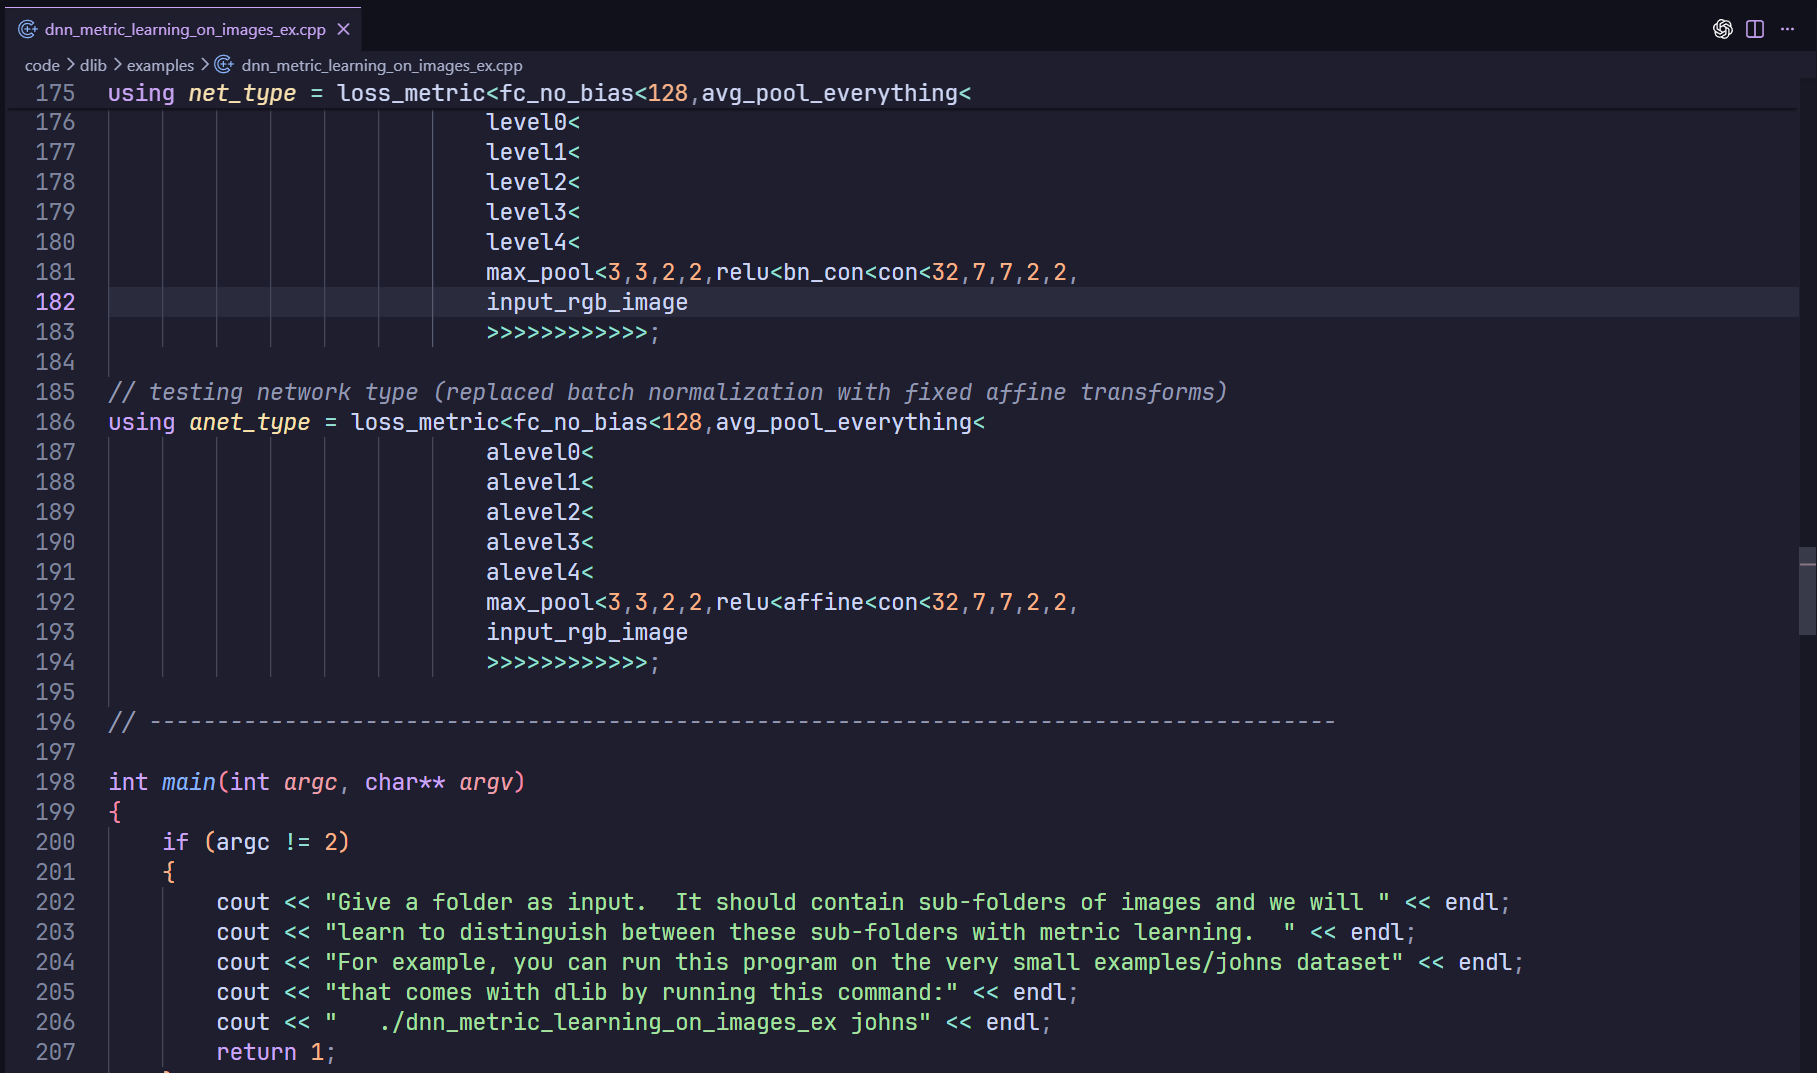
\includegraphics[width=0.86\textwidth]{img/chapter2/dlib_metric_learning_source.png}
  \caption{dlib 度量学习示例源码}
  \label{fig:dlib_metric_learning_source}
\end{figure}

\subsection{示例入口与数据目录组织}

\subsubsection{命令行输入与顶层目录}

dlib 示例要求命令行传入一个顶层目录。该目录下的每个子目录代表一个身份，子目录中放置该身份的多张图片。示例注释中的结构可以概括为：

\begin{minted}{text}
top_level_directory/
  person1/
    image1.jpg
    image2.jpg
  person2/
    image3.jpg
    image4.jpg
\end{minted}

这种结构把身份标签编码在目录层级中。程序并不关心人物目录的具体名称，也不要求图片文件名遵循统一格式；它只利用“同一子目录中的图片属于同一身份”这一事实生成训练标签。这样的数据组织方式简单直观，也便于人工检查数据是否放错目录。

示例中的 \mintinline{cpp}|load_objects_list| 会遍历顶层目录下的所有子目录，并把每个子目录中的图片路径收集成一个 \mintinline{cpp}|std::vector<string>|。最终得到的数据结构是 \mintinline{cpp}|std::vector<std::vector<string>>|：外层向量表示不同身份，内层向量表示某个身份对应的图片列表。后续 mini-batch 采样会直接基于这个结构随机选择身份和图片。

\begin{figure}[htbp]
  \centering
  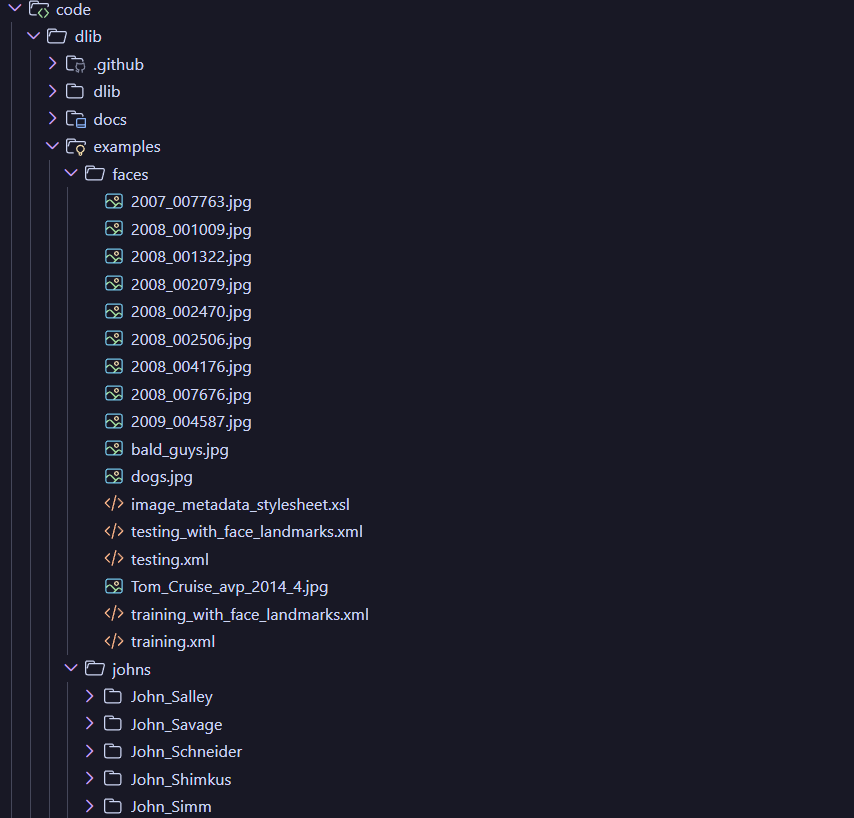
\includegraphics[width=0.86\textwidth]{img/chapter2/dlib_training_dataset_tree.png}
  \caption{dlib 训练数据目录组织}
  \label{fig:dlib_training_dataset_tree}
\end{figure}

\subsubsection{训练数据与参考样本的区别}

dlib 示例中的目录用于训练网络参数。程序会反复读取这些图片，生成 mini-batch，计算损失并更新网络权重。浏览器项目中的 \mintinline{text}|public/img/labeled_images| 虽然也按人物目录组织，但作用不同：它只用于提取参考描述子并构造匹配器，不会更新预训练模型。因此，两者在目录形态上相似，在训练语义上不同。

这个区别很重要。如果把浏览器项目中的注册图片误解为训练集，就会误以为页面可以通过几张图片“训练出”新模型。实际上，页面只是利用已经训练好的描述子网络，把参考图片转换成向量，再把新图片向量与参考向量做距离比较。dlib 示例则展示了描述子网络本身如何通过大量有标签图片训练出来。

\subsection{mini-batch 采样机制}

\subsubsection{度量学习依赖 batch 组成的原因}

普通分类任务的 mini-batch 只需要包含图片和类别标签，模型通过分类损失学习每张图片属于哪个类别。度量学习则更依赖 batch 内部的配对关系。一次训练步骤中，损失函数需要同时看到“应该靠近的样本对”和“应该远离的样本对”。如果 batch 中每个身份只有一张图片，就无法形成同身份正样本对；如果 batch 中身份数量太少，又缺少足够的负样本对。

dlib 示例通过 \mintinline{cpp}|load_mini_batch| 明确控制 batch 组成。函数参数 \mintinline{cpp}|num_people| 表示一次采样多少个不同身份，\mintinline{cpp}|samples_per_id| 表示每个身份采样多少张图片。主训练流程调用 \mintinline{cpp}|load_mini_batch(5, 5, rnd, objs, images, labels)|，即每次选择 5 个身份，每个身份选 5 张图片，共得到 25 张图片。这样，同一身份内部任意两张图片构成正样本对，不同身份之间的图片构成负样本对。

设一次 mini-batch 中选择 $P$ 个身份，每个身份采样 $K$ 张图片，则 batch 大小为

\begin{equation}
  B = P K.
  \label{eq:batch_size}
\end{equation}

在 dlib 示例的设置中，$P=5$、$K=5$，因此 $B=25$。如果只考虑无序样本对，正样本对数量为

\begin{equation}
  N_{+} = P {K \choose 2} = P \frac{K(K-1)}{2},
  \label{eq:positive_pairs}
\end{equation}

负样本对数量为

\begin{equation}
  N_{-} = {P \choose 2}K^2 = \frac{P(P-1)}{2}K^2.
  \label{eq:negative_pairs}
\end{equation}

代入 $P=5$、$K=5$ 可得 $N_{+}=50$、$N_{-}=250$。这说明一次 batch 中可以产生大量配对关系，而不是只产生 25 个独立训练样本。度量学习正是利用这些样本对来塑造嵌入空间。

\begin{figure}[htbp]
  \centering
  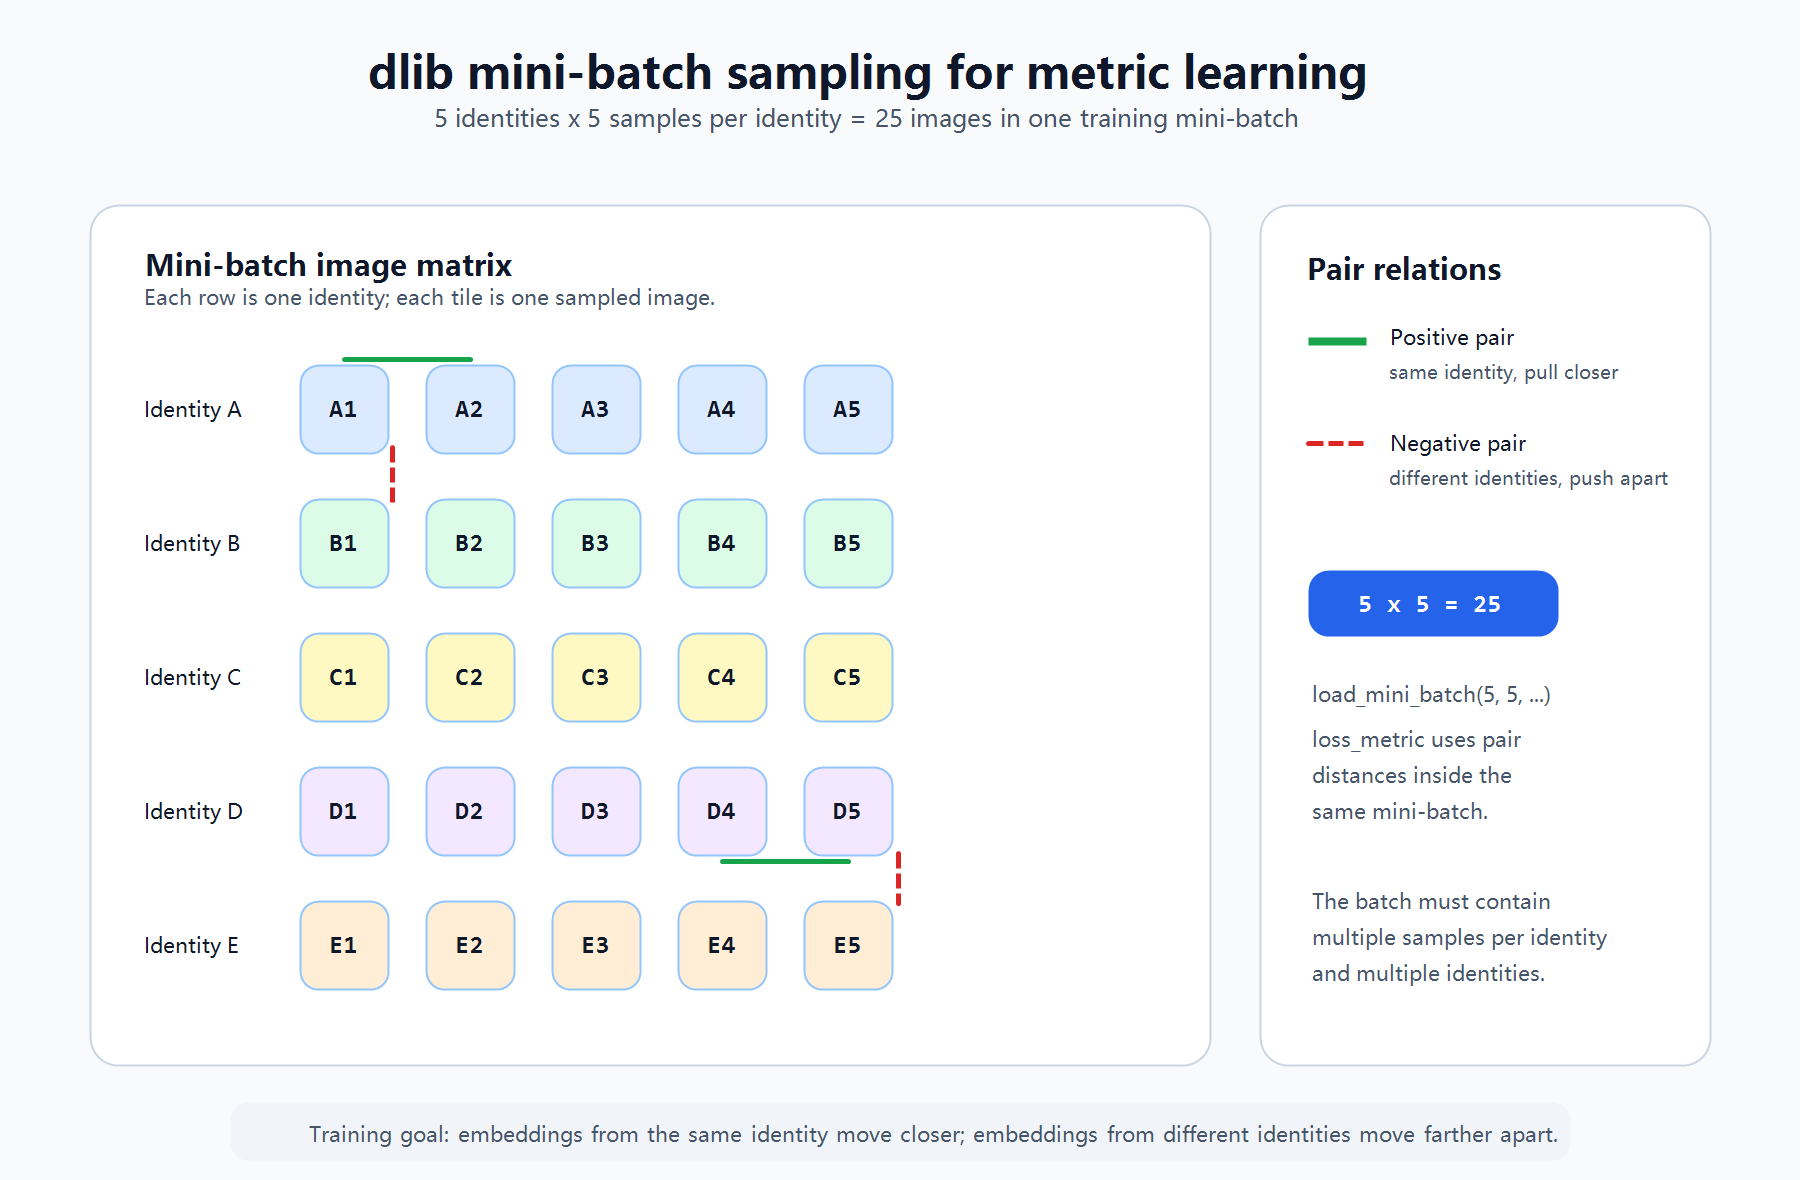
\includegraphics[width=0.88\textwidth]{img/chapter2/dlib_minibatch_sampling.png}
  \caption{深度度量学习 mini-batch 采样示意}
  \label{fig:dlib_minibatch_sampling}
\end{figure}

\subsubsection{随机选择与标签生成}

\mintinline{cpp}|load_mini_batch| 首先清空 \mintinline{cpp}|images| 和 \mintinline{cpp}|labels|，然后用 \mintinline{cpp}|already_selected| 避免同一个身份在一次 batch 中被重复选中。对每个被选中的身份，函数再从该身份图片列表中随机选择 \mintinline{cpp}|samples_per_id| 张图片，调用 \mintinline{cpp}|load_image| 读取图像，并把身份编号写入 \mintinline{cpp}|labels|。

这里的标签是身份在外层向量中的下标，而不是人物姓名字符串。对于训练损失来说，标签只需要表达“相同”或“不同”的关系。只要两张图片标签相同，损失函数就会把它们当作同身份样本；标签不同，就会当作不同身份样本。也就是说，度量学习并不关心类别名称的语义，只关心样本之间的关系。

这一关系可以写成二值函数：

\begin{equation}
  s_{ij} =
  \begin{cases}
    1, & y_i = y_j,\\
    0, & y_i \ne y_j,
  \end{cases}
  \label{eq:pair_label}
\end{equation}

其中 $y_i$ 和 $y_j$ 是两张图片的身份标签。当 $s_{ij}=1$ 时，样本对属于正样本对；当 $s_{ij}=0$ 时，样本对属于负样本对。后续损失函数只需要根据 $s_{ij}$ 的取值决定是拉近距离还是推远距离。

\subsubsection{数据增强与尺寸约束}

采样完成后，示例会对图片进行简单数据增强。代码先调用 \mintinline{cpp}|disturb_colors(crop, rnd)| 扰动颜色，再以较高概率调用 \mintinline{cpp}|jitter_image(crop, rnd)| 对图像做轻微变换。颜色扰动可以模拟亮度、色彩和拍摄环境变化，抖动变换可以让模型对局部位置变化更鲁棒。对于人脸识别而言，同一身份可能出现在不同光照、角度和成像条件下，数据增强有助于模型学习更稳定的身份特征。

示例还强调 batch 中所有图片尺寸必须一致。深度网络的输入张量需要统一高度、宽度和通道数。如果训练集中图片尺寸差异较大，通常要提前裁剪、缩放或对齐。dlib 示例没有把完整的人脸检测对齐流程写入本文件，而是假设输入图片已经适合训练。真实项目中，训练前的数据清洗、裁剪和对齐往往会占据大量工作。

\subsection{网络结构与 128 维描述子}

\subsubsection{ResNet 主体结构}

示例中的网络结构来自 dlib 的 ResNet 示例，并将普通分类损失替换为 \mintinline{cpp}|loss_metric|。代码使用大量类型别名定义残差块和网络层级，例如 \mintinline{cpp}|res|、\mintinline{cpp}|res_down|、\mintinline{cpp}|level0| 到 \mintinline{cpp}|level4|。网络前端包含卷积、ReLU 和池化操作，中间由多级残差结构提取特征，末端通过全局平均池化和全连接层输出固定长度向量。

残差结构的意义在于缓解深层网络训练困难。通过跳跃连接，网络可以学习残差映射，而不是每一层都从零学习完整变换。对于图像识别任务，残差网络能够在较深层级提取从边缘、纹理到面部结构的多层特征。dlib 示例的网络比大型图像分类网络更小，但仍保留了 ResNet 的核心思想。

\begin{figure}[htbp]
  \centering
  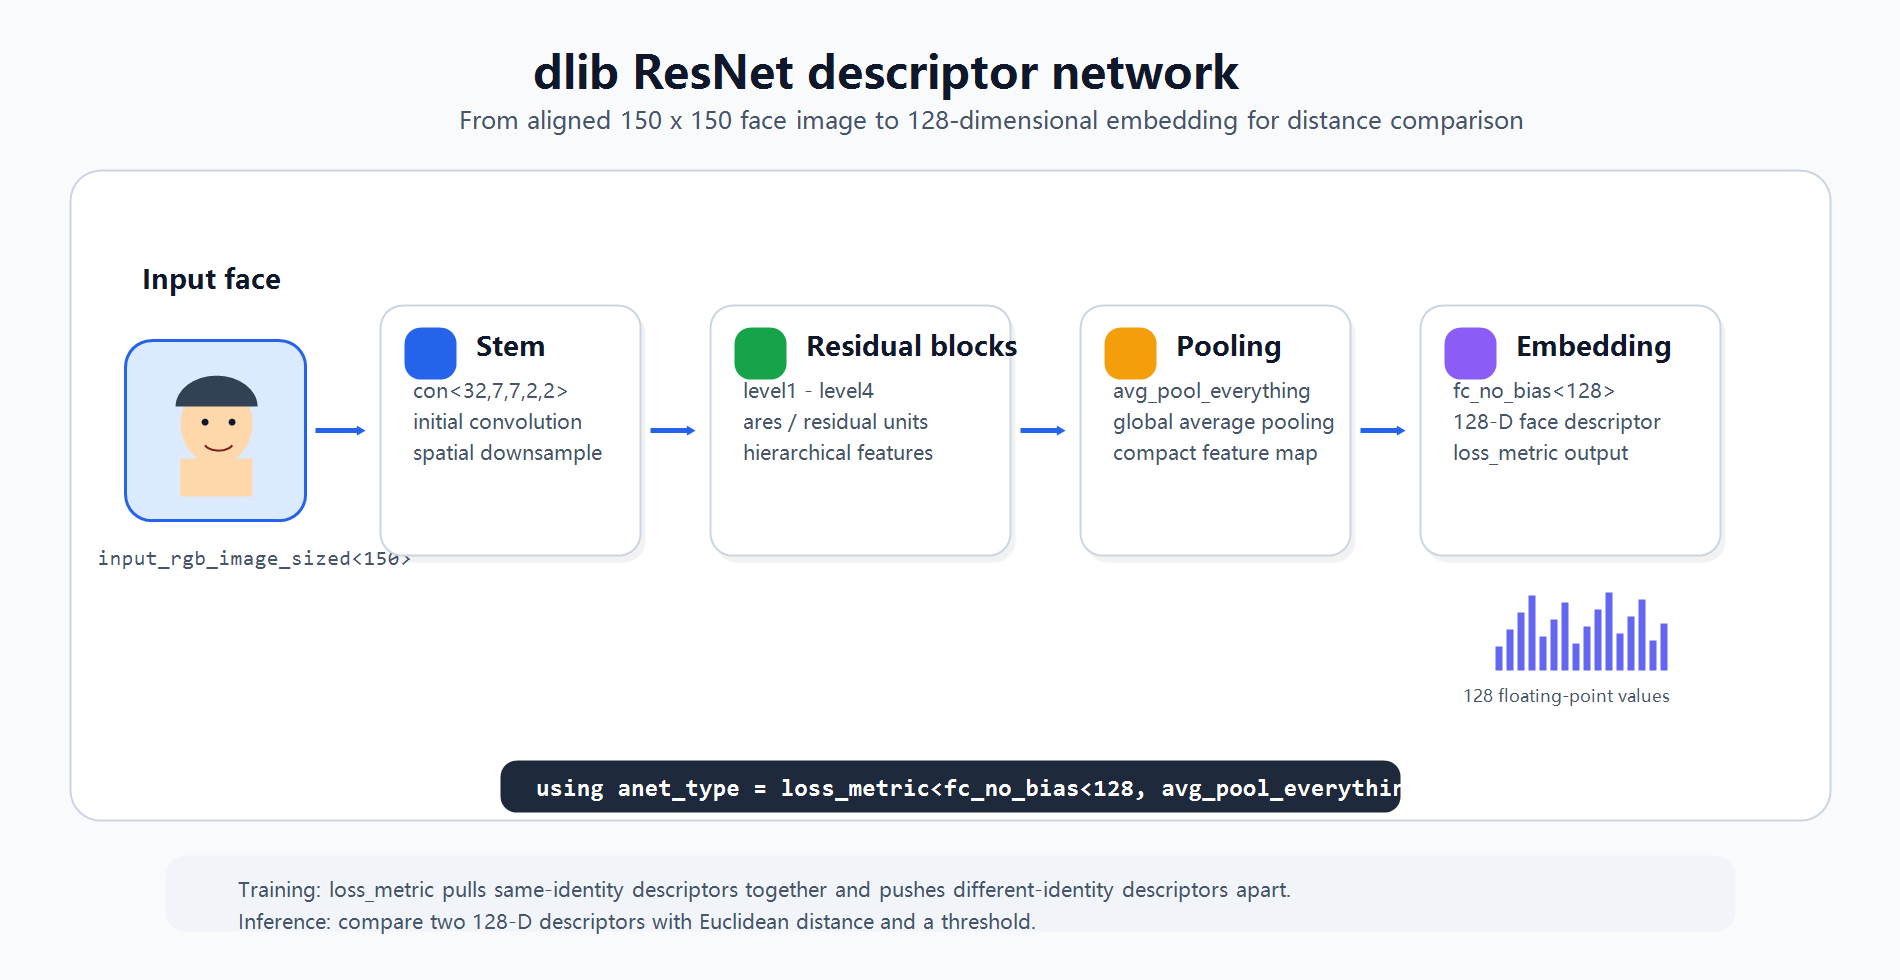
\includegraphics[width=0.92\textwidth]{img/chapter2/dlib_resnet_descriptor_network.png}
  \caption{dlib 人脸描述子网络结构}
  \label{fig:dlib_resnet_descriptor_network}
\end{figure}

\subsubsection{训练网络与测试网络}

示例定义了两个网络类型：\mintinline{cpp}|net_type| 和 \mintinline{cpp}|anet_type|。\mintinline{cpp}|net_type| 用于训练，网络内部使用 \mintinline{cpp}|bn_con| 批归一化层；\mintinline{cpp}|anet_type| 用于测试和推理，把批归一化替换为 \mintinline{cpp}|affine| 固定仿射变换。这样做是因为训练阶段可以使用 batch 统计量，而推理阶段通常希望网络行为固定，不再依赖当前 batch 的均值和方差。

这种训练网络与推理网络的区分体现了深度学习工程中的常见做法。模型训练时为了稳定梯度和加速收敛，可以使用批归一化；模型部署时则需要把训练阶段学到的统计量固化下来，使单张图片或小 batch 输入也能得到稳定输出。浏览器端预训练模型虽然不直接暴露这些 C++ 类型，但同样经历了从训练形态到推理形态的转换。

\subsubsection{128 维输出向量}

网络末端的 \mintinline{cpp}|fc_no_bias<128>| 表示输出 128 维向量，\mintinline{cpp}|avg_pool_everything| 表示在进入全连接层前做全局平均池化。这个 128 维向量就是人脸描述子。描述子不是分类概率，也不是姓名，而是模型为输入人脸生成的紧凑特征表示。

使用固定长度描述子有两个好处。第一，它便于比较。任意两张人脸图片经过同一个网络后都会得到 128 维向量，可以直接计算欧氏距离。第二，它支持开放集识别。系统不需要预先固定所有可能人物类别，只要为新人物保存若干参考描述子，就能通过最近邻或阈值比较进行匹配。这也是它比普通闭集分类更适合人脸识别应用的原因。

\subsection{loss\_metric 损失函数}

\subsubsection{距离关系作为训练目标}

\mintinline{cpp}|loss_metric| 的作用是把样本之间的距离关系写入训练目标。训练时，网络根据标签知道哪些图片属于同一身份，哪些图片属于不同身份。对于同身份样本，损失函数希望它们在嵌入空间中的距离小；对于不同身份样本，损失函数希望它们的距离足够大。随着训练进行，网络逐渐学会把身份相关特征编码进 128 维向量。

这种目标与普通 softmax 分类不同。softmax 分类学习的是“输入属于哪个类别”，通常输出固定类别上的概率分布；度量学习学习的是“输入之间应该如何排列”，输出的是可比较的特征向量。对于人脸识别场景，后者更灵活，因为实际系统经常需要新增从未出现在训练集中的身份。

dlib 的 \mintinline{cpp}|loss_metric| 可以理解为基于样本对的 hinge loss。设距离阈值为 $T$，间隔参数为 $m$。根据 dlib 默认实现，若不手动指定参数，则 $T=0.6$、$m=0.04$。对于同身份样本对，距离应小于阈值附近的安全范围，其损失可写为

\begin{equation}
  L_{ij}^{+} = \max(0, d_{ij} - T + m), \qquad y_i = y_j.
  \label{eq:positive_loss}
\end{equation}

当 $d_{ij}$ 已经足够小，即 $d_{ij} < T-m$ 时，该项损失为 0；当同身份样本距离过大时，损失随距离增大而线性增加，反向传播会推动两个描述子靠近。

对于不同身份样本对，距离应大于阈值附近的安全范围，其损失可写为

\begin{equation}
  L_{ij}^{-} = \max(0, T - d_{ij} + m), \qquad y_i \ne y_j.
  \label{eq:negative_loss}
\end{equation}

当 $d_{ij} > T+m$ 时，不同身份样本已经分得足够开，损失为 0；当不同身份样本距离过近时，损失变为正值，训练过程会推动它们在嵌入空间中分离。综合正负样本对后，一次 mini-batch 的目标可概括为

\begin{equation}
  L =
  \sum_{(i,j)\in \mathcal{P}} L_{ij}^{+}
  +
  \sum_{(i,j)\in \mathcal{N}_{h}} L_{ij}^{-},
  \label{eq:metric_loss}
\end{equation}

其中 $\mathcal{P}$ 表示正样本对集合，$\mathcal{N}_{h}$ 表示被选入损失计算的困难负样本集合。dlib 文档说明，当 batch 中正样本对数量为 $N$ 时，损失层只选取 $N$ 个最难的非匹配样本对参与负样本损失计算。这样可以缓解负样本对数量远多于正样本对造成的不平衡问题。

\subsubsection{嵌入空间的直观理解}

可以把训练后的嵌入空间想象成一个高维坐标系。每张人脸图片经过网络后都会落在这个坐标系中的某个点。同一个人的多张图片虽然拍摄角度、表情和光照不同，但应该落在相近区域；不同人的图片应该落在相对远的区域。识别时，只要比较两个点之间的距离，就可以判断它们是否可能属于同一身份。

因此，理想的嵌入空间应满足如下关系：

\begin{equation}
  \lVert f_\theta(x_i) - f_\theta(x_j) \rVert_2 < T,
  \qquad y_i = y_j,
  \label{eq:same_identity_constraint}
\end{equation}

\begin{equation}
  \lVert f_\theta(x_i) - f_\theta(x_j) \rVert_2 \ge T,
  \qquad y_i \ne y_j.
  \label{eq:different_identity_constraint}
\end{equation}

公式 \ref{eq:same_identity_constraint} 和公式 \ref{eq:different_identity_constraint} 不是要求所有训练样本都能被完美分开，而是表达训练目标的方向。真实数据中存在姿态、遮挡、模糊和身份相似等复杂情况，因此损失函数采用带间隔的软约束，让模型在大量样本对上逐步逼近这种距离结构。

需要强调的是，实际描述子是 128 维，无法直接画在二维平面上。占位图中的二维图只是一种教学示意，用于说明“同类靠近、异类远离”的思想。真实模型中的距离关系由训练数据、网络结构和损失函数共同决定。

\subsection{训练器与优化过程}

\subsubsection{训练器配置}

主函数中先构造 \mintinline{cpp}|net_type net|，再创建 \mintinline{cpp}|dnn_trainer<net_type> trainer(net, sgd(0.0001, 0.9))|。训练器使用随机梯度下降优化网络参数，其中 \mintinline{cpp}|0.0001| 和 \mintinline{cpp}|0.9| 分别对应优化器中的权重衰减和动量设置。随后，代码调用 \mintinline{cpp}|trainer.set_learning_rate(0.1)| 设置初始学习率，并调用 \mintinline{cpp}|trainer.be_verbose()| 输出训练日志。

示例还调用 \mintinline{cpp}|trainer.set_synchronization_file("face_metric_sync", std::chrono::minutes(5))| 定期保存同步文件。同步文件的作用是让训练过程具备一定恢复能力。如果训练耗时很长，中途异常中断时，可以利用同步状态继续训练，而不是完全从头开始。这体现了实际训练工程对可靠性的要求。

\subsubsection{学习率停止条件}

训练循环的停止条件是学习率降到 \mintinline{cpp}|1e-4| 以下。示例中设置这个阈值是为了让示例程序可以较快结束；如果要训练高质量模型，通常需要更充分的数据、更长训练时间和更细致的学习率策略。学习率下降意味着优化过程进入后期，参数更新幅度变小，模型逐渐接近当前设置下的收敛状态。

训练循环本身不断从数据队列中取出图片和标签，然后调用 \mintinline{cpp}|trainer.train_one_step(images, labels)| 完成一次训练步骤。每一步都会前向计算描述子，依据标签计算距离损失，再反向传播更新网络参数。这个过程反复进行，直到学习率降低到停止阈值。

\subsection{主函数训练流程拆解}

\subsubsection{参数检查与数据读入}

示例的 \mintinline{cpp}|main| 函数首先检查命令行参数数量。如果没有传入训练数据目录，程序会输出用法说明并结束。这说明训练程序把数据路径作为外部输入，而不是写死在源码中。随后，程序调用 \mintinline{cpp}|load_objects_list(argv[1])| 读取顶层目录，并输出 \mintinline{cpp}|objs.size()|，用于确认当前数据集中包含多少个身份。

这一输出虽然简单，但在实验复现中很有价值。如果 \mintinline{cpp}|objs.size()| 为 0 或明显小于预期，说明训练目录结构不正确，可能是路径传错、子目录为空，或者图片没有被识别为有效文件。训练前先检查身份数量，可以避免程序进入后续训练后才发现数据无效。

\subsubsection{训练对象初始化}

读取数据后，程序构造 \mintinline{cpp}|net_type net| 作为待训练网络，再创建 \mintinline{cpp}|dnn_trainer|。训练器绑定到网络对象，因此后续所有梯度更新都会作用在 \mintinline{cpp}|net| 上。随后，程序设置学习率、日志输出和同步文件。这些配置共同定义了训练过程的外部行为：学习率决定更新步幅，日志用于观察训练进度，同步文件用于恢复。

从工程角度看，这一阶段相当于训练任务的初始化。只有网络、优化器、学习率、数据列表和同步策略都准备好，程序才真正进入训练循环。课程报告中把这一阶段写清楚，可以帮助读者理解训练程序并不是一上来就“训练模型”，而是先建立数据和优化环境。

\subsubsection{生产者消费者训练循环}

主训练循环没有直接调用 \mintinline{cpp}|load_mini_batch|，而是从 \mintinline{cpp}|qimages| 和 \mintinline{cpp}|qlabels| 两个管道中取数据。数据加载线程负责生产 batch，训练主线程负责消费 batch。核心步骤可以概括为：加载线程读取图片并生成标签，放入队列；训练线程从队列取出图片和标签；训练器执行 \mintinline{cpp}|train_one_step| 更新网络参数。

这种结构把 I/O 和计算分离。对于大规模图片训练，如果没有数据加载队列，训练线程可能频繁等待磁盘和 CPU 图像解码；有了队列之后，只要加载速度足够快，训练线程就能持续获得 batch。示例虽然是教学代码，但已经体现了真实训练系统常用的流水线思想。

\subsection{多线程数据加载}

\subsubsection{为什么需要异步加载}

深度学习训练不只消耗 GPU 计算，也消耗 CPU 读取、解码和增强图片的能力。如果训练线程每次都等待磁盘读取和图像处理，GPU 可能处于空闲状态。为了提高吞吐量，dlib 示例使用 \mintinline{cpp}|dlib::pipe| 和多个数据加载线程，让数据加载与训练计算并行进行。

示例创建了两个管道：\mintinline{cpp}|qimages| 用于传递图片 batch，\mintinline{cpp}|qlabels| 用于传递标签 batch。数据加载线程不断调用 \mintinline{cpp}|load_mini_batch| 生成图片和标签，再把它们放入队列；训练主线程从队列中取出 batch 并执行训练。这个模式可以概括为“加载线程生产数据，训练线程消费数据”。

\subsubsection{线程数量与资源平衡}

示例启动了 5 个数据加载线程，并在注释中提示线程数量应根据 CPU 核心数调整。线程过少可能无法及时提供数据，导致训练等待；线程过多则可能造成 CPU 竞争、内存占用增加和上下文切换开销。真实训练任务需要根据数据集大小、磁盘速度、CPU 核心数和 GPU 性能进行平衡。

这部分代码说明，训练一个人脸描述子模型并不是只有网络结构和损失函数。数据加载、增强、队列缓冲、线程同步和异常处理都会影响训练效率。相比之下，浏览器项目只执行推理，不承担这些训练工程复杂度，因此前端页面显得更轻量。

\begin{figure}[htbp]
  \centering
  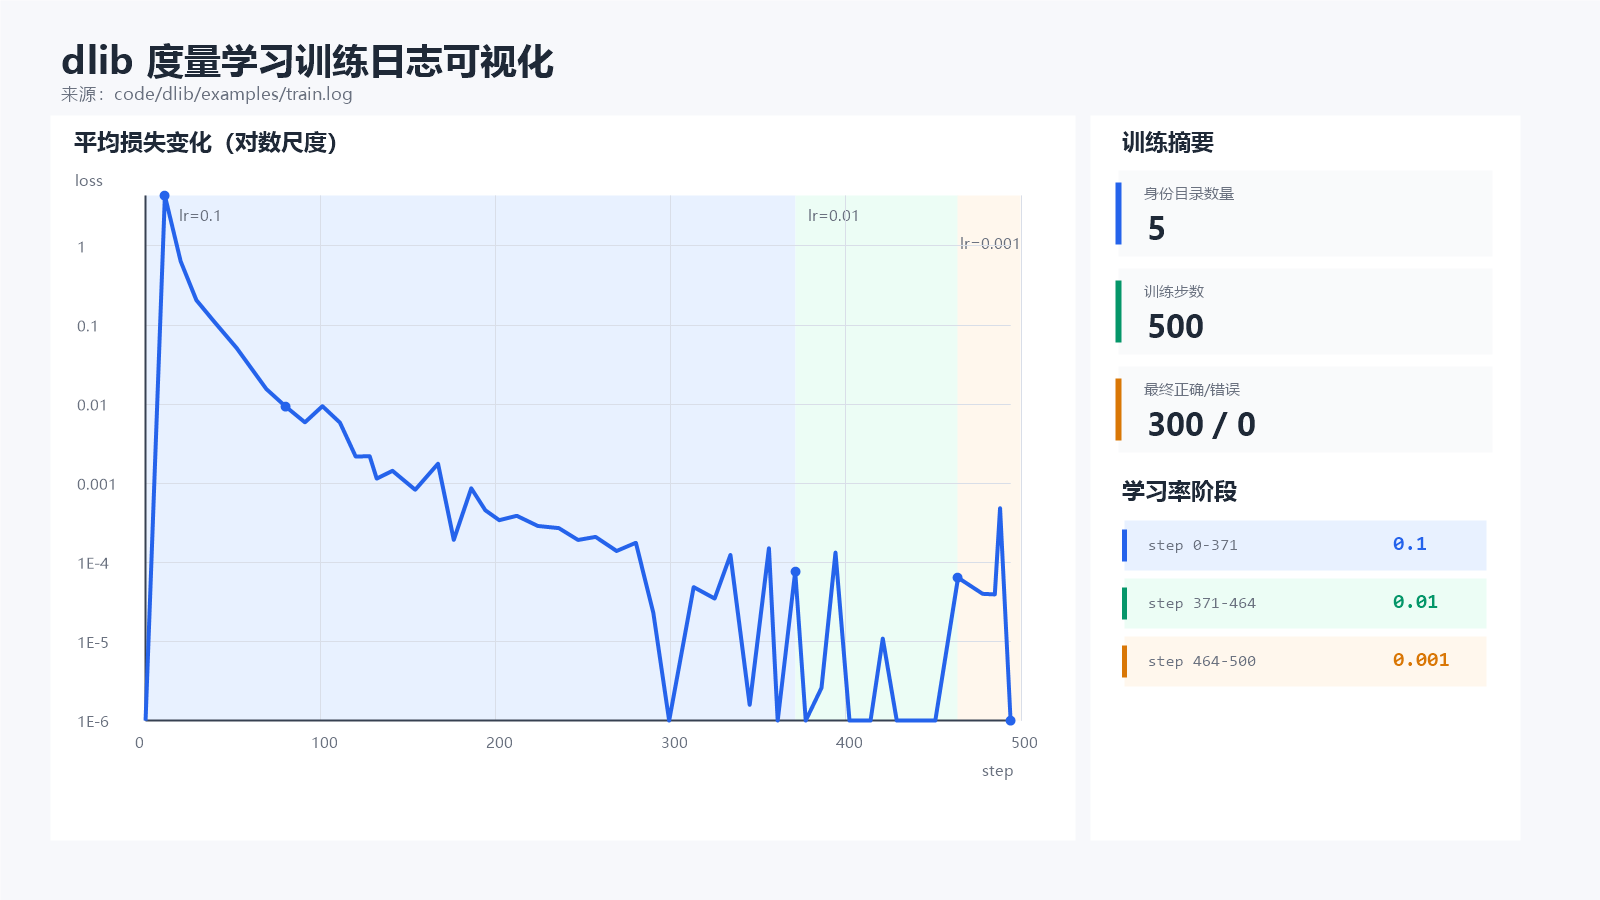
\includegraphics[width=0.94\textwidth]{img/chapter2/dlib_training_log.png}
  \caption{dlib 度量学习训练日志可视化}
  \label{fig:dlib_training_log}
\end{figure}

图 \ref{fig:dlib_training_log} 根据本次运行生成的 \path{code/dlib/examples/train.log} 绘制。日志显示，训练数据中共有 5 个身份目录，训练过程共执行 500 个 step。平均损失在前期迅速下降，随后学习率从 0.1 依次降低到 0.01 和 0.001，说明训练器在后期逐步减小参数更新幅度。训练结束后的简单配对验证结果为 \mintinline{text}|num_right: 300|、\mintinline{text}|num_wrong: 0|，表示当前随机 batch 中 300 个样本对均被阈值规则正确区分。

为了便于对照图中的曲线和学习率阶段，训练日志中的关键片段如下：

\begin{minted}{text}
objs.size(): 5
step#: 11    learning rate: 0.1    average loss: 4.33944
step#: 80    learning rate: 0.1    average loss: 0.00936225
step#: 371   learning rate: 0.01   average loss: 7.73552e-05
step#: 464   learning rate: 0.001  average loss: 6.41373e-05
training steps: 500
done training
num_right: 300
num_wrong: 0
\end{minted}

\subsection{WSL 环境下的示例编译与运行记录}

\subsubsection{创建构建目录并生成工程}

为了验证 dlib 官方示例能够在本地环境中运行，本实验在 WSL 环境下进入 \mintinline{text}|code/dlib/examples| 目录，并单独创建 \mintinline{text}|build-wsl| 作为构建目录。这样可以把 CMake 生成的中间文件与示例源码分离，便于后续重新构建和清理。实际执行的命令如下：

\begin{minted}{bash}
mkdir build-wsl
cd build-wsl
cmake .. -DCMAKE_BUILD_TYPE=Release
\end{minted}

其中，\mintinline{bash}|cmake ..| 表示以上一级目录中的 \mintinline{text}|CMakeLists.txt| 作为工程入口，\mintinline{bash}|-DCMAKE_BUILD_TYPE=Release| 用于生成发布配置，使后续训练程序以优化后的方式编译。图 \ref{fig:wsl_cmake_configure} 展示了创建构建目录并执行 CMake 配置的过程。

\begin{figure}[htbp]
  \centering
  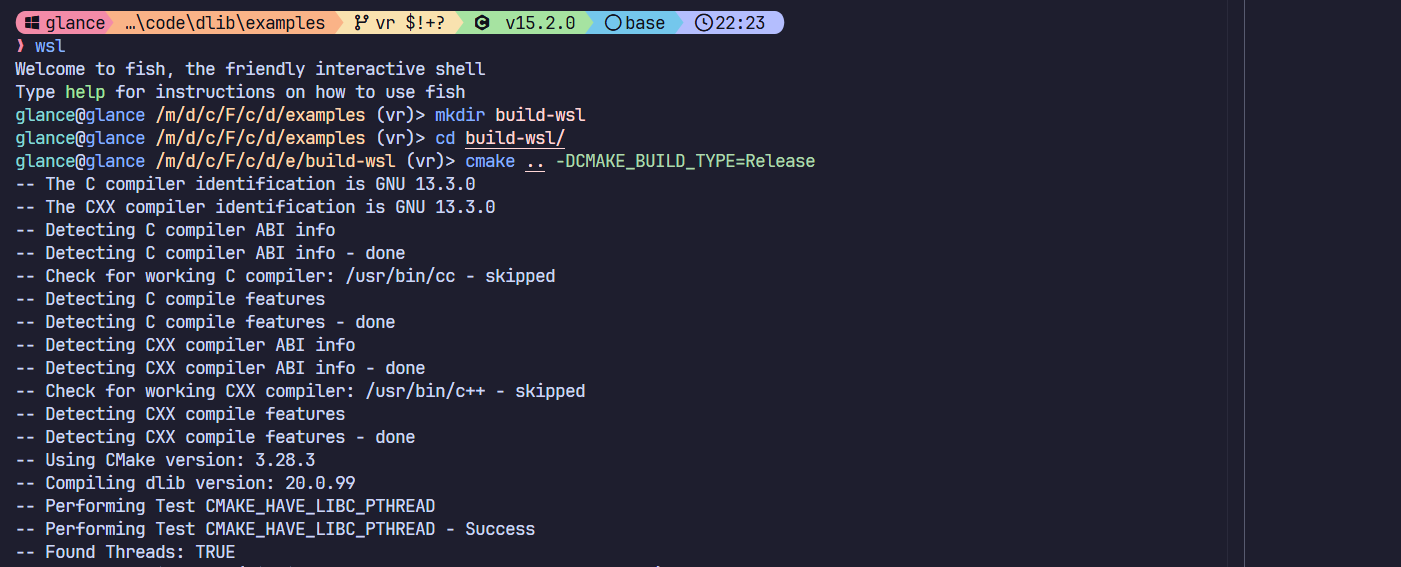
\includegraphics[width=0.9\textwidth]{img/chapter2/使用wsl编译1.png}
  \caption{WSL 环境下创建 build-wsl 目录并执行 CMake 配置}
  \label{fig:wsl_cmake_configure}
\end{figure}

\subsubsection{编译度量学习示例目标}

CMake 配置完成后，需要在构建目录中编译具体示例目标。这里选择的目标是 \mintinline{text}|dnn_metric_learning_on_images_ex|，对应本章分析的 \path{dlib/examples/dnn_metric_learning_on_images_ex.cpp}。编译命令如下：

\begin{minted}{bash}
cmake --build . --target dnn_metric_learning_on_images_ex -j4
\end{minted}

其中，\mintinline{bash}|--build .| 表示在当前构建目录中执行构建，\mintinline{bash}|--target dnn_metric_learning_on_images_ex| 指定只编译度量学习示例，\mintinline{bash}|-j4| 表示使用 4 个并行任务加快编译速度。图 \ref{fig:wsl_cmake_build_target} 展示了该目标的编译过程。

\begin{figure}[htbp]
  \centering
  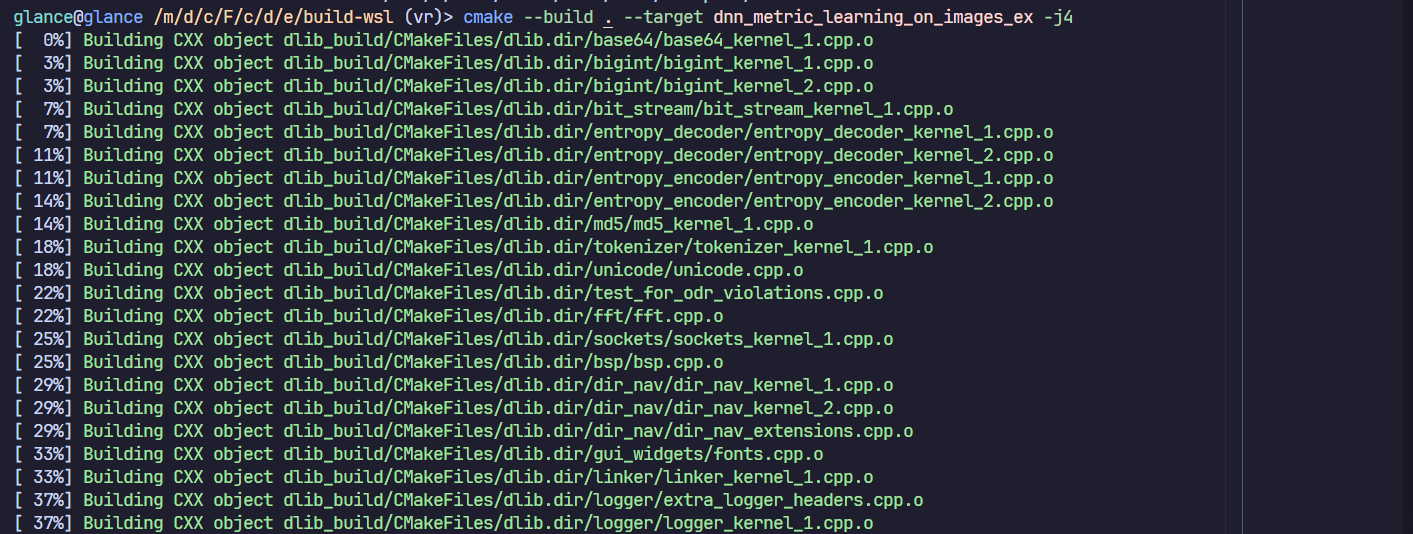
\includegraphics[width=0.9\textwidth]{img/chapter2/使用wsl编译2.png}
  \caption{使用 CMake 编译 dnn\_metric\_learning\_on\_images\_ex 示例目标}
  \label{fig:wsl_cmake_build_target}
\end{figure}

\subsubsection{返回 examples 目录并运行训练}

示例程序编译完成后，实验返回上一级 \mintinline{text}|examples| 目录，并启动训练相关命令。截图中的执行过程如下：

\begin{minted}{bash}
cd ..
cmake --build . --target dnn_metric_learning_on_images_ex -j4
\end{minted}

这一阶段的重点是从构建结果进入示例运行流程，观察程序是否能够正常加载训练数据、输出训练日志并进入优化过程。图 \ref{fig:wsl_training_start} 展示了返回目录后继续执行示例目标的过程。

\begin{figure}[htbp]
  \centering
  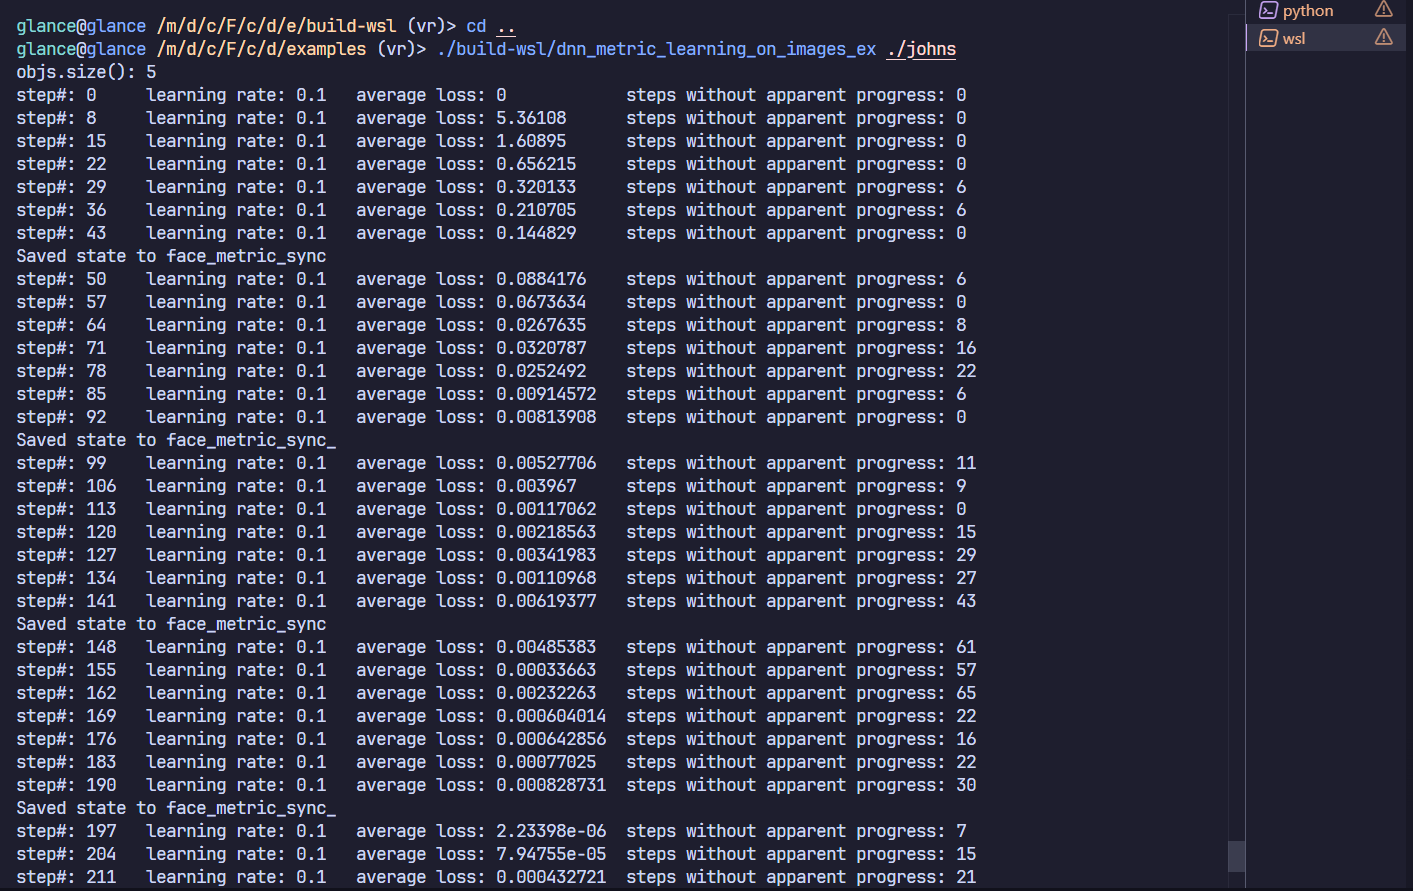
\includegraphics[width=0.9\textwidth]{img/chapter2/使用wsl编译3.png}
  \caption{返回 examples 目录后继续执行度量学习示例}
  \label{fig:wsl_training_start}
\end{figure}

训练过程结束后，终端会输出训练完成信息，并保存训练得到的模型文件。图 \ref{fig:wsl_training_finished} 展示了本次运行结束时的终端状态。结合前文对训练循环的分析可以看出，命令行中的输出对应了数据读取、mini-batch 训练、学习率变化、模型清理和序列化保存等步骤。

\begin{figure}[htbp]
  \centering
  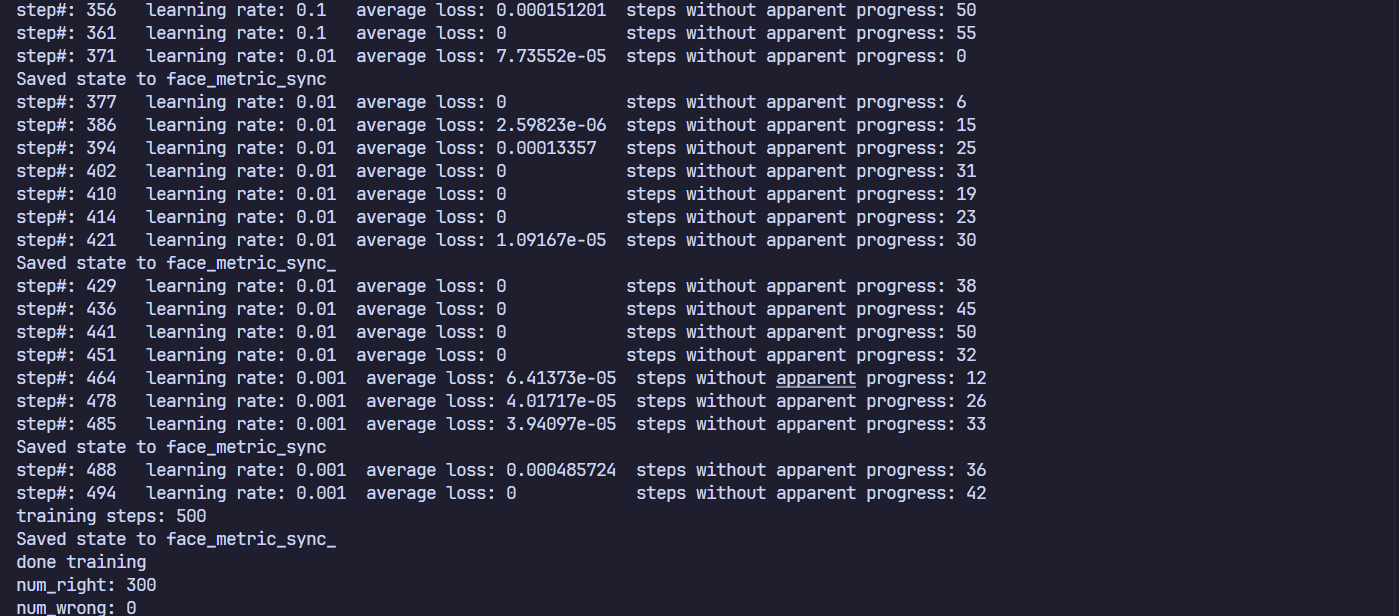
\includegraphics[width=0.9\textwidth]{img/chapter2/使用wsl编译4.png}
  \caption{dlib 度量学习示例训练结束}
  \label{fig:wsl_training_finished}
\end{figure}

\subsection{训练数据准备与质量控制}

\subsubsection{身份数量与样本数量}

度量学习模型的效果高度依赖训练数据。首先，身份数量必须足够多。如果只有少量身份，模型很难学习到具有泛化能力的身份区分特征。其次，每个身份需要多张图片。如果每个身份只有一张图，模型无法学习同一身份在不同姿态、表情和光照下的变化范围。示例中每个 batch 采样 5 个身份、每个身份 5 张图片，正是为了在一次训练步骤中同时呈现身份内变化和身份间差异。

训练数据还需要避免严重不均衡。如果某些身份图片很多，而另一些身份只有一两张，随机采样可能让模型更多看到样本丰富的身份。示例按身份随机选择，再按身份内图片随机选择，可以在一定程度上控制 batch 中身份分布，但数据集本身仍应尽量保证每个身份有足够样本。

\subsubsection{图片质量与预处理}

训练图片最好满足清晰、对齐、主体明确和尺寸一致等条件。如果图片中人脸位置差异过大，模型可能把背景、姿态或裁剪方式当成身份特征，从而降低泛化能力。真实训练流程通常会先用人脸检测器找到人脸区域，再根据关键点进行对齐和裁剪，使眼睛、鼻子、嘴巴等结构落在相对稳定的位置。

dlib 示例关注度量学习训练本身，没有完整展开人脸检测和对齐流程。因此，在课程报告中应说明：该示例适合理解训练机制，但真实人脸识别系统还需要前置数据清洗。数据清洗包括删除非人脸图片、剔除错误身份目录、统一图像尺寸、处理重复图片、检查严重模糊和遮挡样本等。

\subsubsection{数据增强的作用边界}

数据增强可以提升模型鲁棒性，但不能替代真实数据多样性。颜色扰动和图像抖动能模拟一定范围内的拍摄变化，但如果训练集中缺少侧脸、不同年龄、不同肤色、不同光照或不同设备来源的数据，模型仍可能在这些场景中表现较差。增强方法只能在已有数据分布附近扩展样本，不能凭空创造完整的现实变化。

因此，训练数据准备应同时关注数量、质量和覆盖范围。对于课程实验，可以不实际训练大模型，但报告中要认识到：模型性能不是由网络结构单独决定的，数据本身同样决定了描述子空间能否泛化到新图片。

\subsection{模型保存与训练后验证}

\subsubsection{模型清理与序列化}

训练结束后，程序调用 \mintinline{cpp}|trainer.get_net()| 等待训练线程状态同步，然后输出训练完成信息。接着，代码调用 \mintinline{cpp}|net.clean()| 清理训练过程中不再需要的临时状态，最后执行 \mintinline{cpp}|serialize("metric_network_renset.dat") << net| 将网络保存到磁盘。保存后的文件可以在后续程序中反序列化加载，用于提取人脸图像的 128 维描述子。

这里需要注意文件名中的 \mintinline{text}|renset| 拼写来自示例代码本身。报告分析时应保持与源码一致，不主动改成 \mintinline{text}|resnet|，否则读者对照代码时会困惑。模型保存步骤标志着训练阶段产物形成，后续应用阶段只需加载该产物执行推理。

\subsubsection{训练后验证流程}

示例最后没有只停留在保存模型，而是继续演示如何使用训练好的网络。程序重新采样一个 mini-batch，将训练网络赋值给测试网络 \mintinline{cpp}|anet_type testing_net = net|，然后调用 \mintinline{cpp}|testing_net(images)| 得到所有图片的嵌入向量。接着，程序两两比较向量距离，统计判断正确的样本对数量。

如果两张图片标签相同，它们的向量距离应该小于阈值；如果标签不同，距离应该大于或等于阈值。这个验证流程虽然比较简单，但清楚展示了度量学习模型的使用方式：模型负责输出描述子，判别逻辑通过距离和阈值完成。

\subsection{距离阈值与开放集识别}

\subsubsection{阈值来源}

示例使用 \mintinline{cpp}|testing_net.loss_details().get_distance_threshold()| 取得距离阈值。这个阈值来自 \mintinline{cpp}|loss_metric| 的距离约束。训练过程中，损失函数会围绕这个距离目标调整向量空间，使同身份样本倾向于落在阈值以内，不同身份样本倾向于落在阈值以外。

阈值判断是人脸识别系统的重要环节。如果阈值设置过大，不同身份可能被误判为同一人；如果阈值设置过小，同一身份在姿态、光照变化较大时可能被误判为不同人。实际应用通常需要在验证集上评估误识率和拒识率，再根据应用场景选择合适阈值。安全要求高的场景往往倾向于更严格阈值，便利性要求高的场景可能接受更宽松阈值。

\subsubsection{与闭集分类的区别}

开放集识别意味着测试阶段可能出现训练阶段没有见过的人。度量学习天然适合这种场景，因为模型输出的是通用描述子，而不是固定类别概率。新增人物时，只需要采集若干参考图片，提取描述子并存入数据库；识别时，将新图片描述子与数据库中的参考描述子比较即可。

闭集分类则假设所有可能类别都在训练集中。它适合固定类别任务，例如识别有限种物体；但在人脸识别中，新增身份非常常见。如果每新增一个人都重新训练输出层，工程成本会很高。因此，dlib 示例展示的描述子加距离匹配思想，更符合人脸识别系统的扩展需求。

\subsection{验证指标与阈值选择}

\subsubsection{num\_right 与 num\_wrong 的含义}

示例在训练后验证阶段定义了 \mintinline{cpp}|num_right| 和 \mintinline{cpp}|num_wrong| 两个计数器。程序遍历当前 mini-batch 中所有图片对，如果两张图片标签相同且距离小于阈值，则计为正确；如果两张图片标签不同且距离大于或等于阈值，也计为正确。相反，同身份距离过大或不同身份距离过小都会计为错误。

这个验证方式可以直观展示描述子空间是否符合训练目标。若 \mintinline{cpp}|num_right| 较多、\mintinline{cpp}|num_wrong| 较少，说明当前 batch 上同身份与不同身份的距离关系较好。不过，这只是对一个随机 mini-batch 的简单检查，不能代替完整测试集评估。真正可靠的模型评估需要在独立数据集上统计更多指标。

\subsubsection{正负样本对的数量}

在一次 \mintinline{cpp}|load_mini_batch(5, 5)| 中，共有 25 张图片。每个身份 5 张图片，因此每个身份内部可以形成 $5 \times 4 / 2 = 10$ 个正样本对，5 个身份共形成 50 个正样本对。不同身份之间的负样本对数量更多：任意两个身份之间有 $5 \times 5 = 25$ 对，5 个身份两两组合共有 $5 \times 4 / 2 = 10$ 组，因此负样本对共 250 对。

这说明度量学习 batch 中负样本对通常远多于正样本对。损失函数需要在大量负样本中找到对训练有帮助的关系，同时保持同身份样本紧密。实际训练中，样本挖掘策略、batch 组成和阈值设置都会影响训练效果。示例采用较简单的随机采样方式，适合教学理解。

\subsubsection{阈值调节的取舍}

阈值选择本质上是在误识和拒识之间取舍。误识是把不同身份判断为同一人，拒识是把同一身份判断为不同人。降低阈值通常会减少误识，但增加拒识；提高阈值通常会减少拒识，但增加误识。不同应用对两类错误的容忍度不同，因此不能只说某个阈值“最好”，而应结合应用场景选择。

例如，在门禁或支付等安全场景中，误识可能造成更严重后果，因此阈值应更严格；在照片聚类或相册整理场景中，偶尔把同一人拆成两个簇的代价较低，可以使用相对宽松的策略，再允许用户手动修正。课程实验中应重点说明阈值的作用和取舍，而不是把某个固定阈值视为普遍适用。

\subsection{与浏览器实验的对应关系}

dlib 示例可以帮助澄清浏览器实验中容易混淆的几个概念。第一，训练数据用于更新网络参数，参考样本用于登记待识别人物；第二，模型输出的人脸描述子是向量，不是姓名；第三，识别结果来自距离比较，而不是模型直接输出人物名称；第四，训练阶段需要处理 mini-batch、数据增强、损失函数、学习率和模型保存，推理阶段则主要处理模型加载、输入转换、描述子提取和结果展示。

浏览器项目中的 \mintinline{javascript}|FaceMatcher| 可以理解为度量学习思想在推理端的简化使用。它并不训练网络，而是接收若干 \mintinline{javascript}|LabeledFaceDescriptors|，在新图片描述子到来时计算距离并返回最接近的标签。dlib 示例则说明这些描述子为什么具有可比较性：因为训练阶段已经通过 \mintinline{cpp}|loss_metric| 让同身份向量靠近、不同身份向量远离。

把训练端和推理端连起来看，可以得到较完整的人脸识别链路：训练阶段学习特征空间，推理阶段加载已经训练好的网络，将输入图片转换为描述子，再通过距离比较得到匹配结果。dlib 示例重点揭示了描述子空间的形成过程，而浏览器实验则展示了预训练描述子模型在页面中的调用方式。

\subsection{实验启示与局限}

dlib 示例虽然展示了完整训练框架，但它仍然是教学示例，而不是可直接用于生产的人脸识别系统。真实系统需要更大规模、更干净、更均衡的数据集，需要严格的人脸检测、对齐和质量控制流程，也需要在独立验证集上评估模型性能。训练后的描述子模型还需要考虑跨年龄、跨光照、跨设备、跨姿态和遮挡条件下的泛化能力。

此外，人脸识别具有明显的隐私和安全属性。训练数据必须来自合法、合规、授权的来源；模型应用也应限制在明确告知和必要范围内。课程报告分析算法流程时，也应避免把技术可行性等同于应用合理性。特别是身份识别系统，一旦用于门禁、考勤、支付或风控等场景，就必须考虑误识、拒识、偏差、数据泄露和用户权利等问题。

从学习角度看，dlib 示例最值得借鉴的是方法论：用目录组织身份数据，用 mini-batch 同时提供正负样本关系，用 ResNet 提取图像特征，用 \mintinline{cpp}|loss_metric| 约束嵌入距离，用阈值完成训练后验证。这些步骤构成了人脸描述子模型训练的基本骨架。理解这个骨架后，再看浏览器端的预训练模型推理，就能更清楚地理解模型能力与匹配逻辑之间的关系。

\subsection{本章小结}

本章围绕 dlib 官方示例 \path{code/dlib/examples/dnn_metric_learning_on_images_ex.cpp}，分析了深度度量学习在人脸识别中的训练流程。示例通过按身份组织图片、构造包含多个身份和多张图片的 mini-batch、使用数据增强提升鲁棒性、采用 ResNet 主体网络输出 128 维描述子，并通过 \mintinline{cpp}|loss_metric| 约束同身份和不同身份样本之间的距离。

训练完成后，模型被序列化保存，并可以通过描述子距离和阈值进行验证。这种“描述子提取 + 距离判断”的思想解释了人脸识别系统为什么不必把每个人都作为固定分类类别，也解释了浏览器实验中注册样本和 \mintinline{javascript}|FaceMatcher| 的作用。至此，报告能够从模型训练和前端推理两个层面说明人脸分析系统的整体工作方式。
